%% abtex2-modelo-trabalho-academico.tex, v-1.9.2 laurocesar
%% Copyright 2012-2017 by abnTeX2 group at http://abntex2.googlecode.com/ 
%%
%% This work may be distributed and/or modified under the
%% conditions of the LaTeX Project Public License, either version 1.3
%% of this license or (at your option) any later version.
%% The latest version of this license is in
%%   http://www.latex-project.org/lppl.txt
%% and version 1.3 or later is part of all distributions of LaTeX
%% version 2005/12/01 or later.
%%
%% This work has the LPPL maintenance status `maintained'.
%% 
%% The Current Maintainer of this work is Emílio Eiji Kavamura,
%% eek.edu@outlook.com; emilio.kavamura@ufpr.br
%% Further information about abnTeX2 are available on 
%%
%% http://abntex2.googlecode.com/
%%
%% https://code.google.com/p/abntex2/issues/ 
%%
%% Further information about UFPR abnTeX2 are available on 
%%
%% https://github.com/eekBR/ufpr-abntex/
%%
%% This work consists of the files 
% 
%          main.tex   programa principal
%      00-dados.tex   entrada de dados 
%    00-pacotes.tex   pacotes carregados no modelo
% 00-pretextual.tex   processamento dos elementos pre-textuais
%          UFPR.sty   ajusta do modelo canonico às normas  UFPR
%
%    referencias.bib
%                     e outras arquivos de imagens
%
%
%------------------------------------------------------------------------
% ------------------------------------------------------------------------
% abnTeX2: Modelo de Trabalho Academico (tese de doutorado, dissertacao de
% mestrado e trabalhos monograficos em geral) em conformidade com 
% ABNT NBR 6023:2018: Informação e documentação - Referências - Elaboração
% ------------------------------------------------------------------------
% ------------------------------------------------------------------------
%
% DATA DE ATUALIZAÇÃO: 2020-06-10

\documentclass[
        % -- opções da classe memoir --
        12pt,                           % tamanho da fonte
        openright,                      % capítulos começam em pág ímpar (insere página vazia caso preciso)
        %twoside,                        % para impressão em verso e anverso. Oposto a oneside
        oneside,
        a4paper,                        % tamanho do papel. 
        % -- opções da classe abntex2 --
        chapter=TITLE,         % títulos de capítulos convertidos em letras maiúsculas
        section=TITLE,         % títulos de seções convertidos em letras maiúsculas
        subsection=Title,      % títulos de subseções convertidos em letras maiúsculas
        %subsubsection=TITLE,  % títulos de subsubseções convertidos em letras maiúsculas
        % -- opções do pacote babel --
        english,                        % idioma adicional para hifenização
        %french,                         % idioma adicional para hifenização
        spanish,                        % idioma adicional para hifenização
        portugues,                      % o último idioma é o principal do documento
        %%%%%%%%%%%%
        %eek: colocação da opção para o sumario ter formatação tradicional
        sumario=tradicional             % título no formato tradicional
        ]{abntex2}


\usepackage{UFPR}
% Pacotes básicos 
% ----------------------------------------------------------
\usepackage{lmodern}			% Usa a fonte Latin Modern			
\usepackage[T1]{fontenc}		% Selecao de codigos de fonte.
\usepackage[utf8]{inputenc}		% Codificacao do documento (conversão automática dos acentos)
\usepackage{lastpage}			% Usado pela Ficha catalográfica
\usepackage{indentfirst}		% Indenta o primeiro parágrafo de cada seção.
\usepackage{color}		    	% Controle das cores
\usepackage{graphicx}			% Inclusão de gráficos
\usepackage{microtype} 			% para melhorias de justificação
\usepackage{ifthen}		    	% para montar condicionais
\usepackage[brazil]{babel}		% para utilizar termos em portugues
\usepackage[final]{pdfpages}    % para incluir páginas de arquivos pdf
\usepackage{lipsum}				% para geração de dummy text
\usepackage{csquotes}

%\usepackage[style=long]{glossaries}
%\usepackage{abntex2glossaries}

\usepackage{algorithm} 
\usepackage{algpseudocode} 
\usepackage{cancel} 		% permite representar o cancelamento de termos em texto ou equacoes	
\usepackage{xcolor} 		% cores extendidas	
\usepackage{smartdiagram}   	% gera diagramas a partir de listas
%\usepackage{float} 		% Para a figura ficar na posição correta	    
\usepackage{textcomp} 		% supporte para fontes da Text Companion 
\usepackage{longtable}		% uso de longtable
\usepackage{amsmath}		% simbolos matematicos
\usepackage{lscape}		% páginas em paisagem
\usepackage{multicol}		% mescla de colunas em tabelas
\usepackage{multirow}		% mescla de linhas em tabelas
\usepackage{newfloat} 		% criação do indice de quadros
%\usepackage{caption} 		% configura legenda 
	%[format=plain]
	%\renewcommand\caption[1]{%
    	%\captionsetup{font=small}	% tamanho da fonte 10pt
    	%,format=hang
 	% \caption{#1}}
	%\captionsetup{width=0.8\textwidth}
\captiondelim{-- }
\captiontitlefont{\small}
\captionnamefont{\small}

\definecolor{dkgreen}{rgb}{0,0.6,0}
\definecolor{gray}{rgb}{0.5,0.5,0.5}
\definecolor{mauve}{rgb}{0.58,0,0.82}

% Pacotes de citações BibLaTeX
% ----------------------------------------------------------
\usepackage[style=abnt,
	backref=true,
	backend=biber,
	citecounter=true,
	backrefstyle=three, 
	url=true,
	maxbibnames=99,
    mincitenames=1,
    maxcitenames=2,
    backref=true,
    hyperref=true,
    firstinits=true,
    uniquename=false,
    uniquelist=false]{biblatex}
    
% Espaçamento entre os itens nas referências (espço de uma linha simples)
% ----------------------------------------------------------
\setlength\bibitemsep{\baselineskip}

% Texto padrão para as referências
% ----------------------------------------------------------
\DefineBibliographyStrings{brazil}{%
	 backrefpage  = {Citado \arabic{citecounter} vez na página},		% originally "cited on page"
	 backrefpages = {Citado \arabic{citecounter} vezes nas páginas},	% originally "cited on pages"
	 urlfrom      = {Dispon\'ivel em},
}

% Ajusta indentação de Referencias no ToC
% ----------------------------------------------------------
\defbibheading{bay}[\bibname]{%
  \chapter*{#1}%
  \markboth{#1}{#1}%
  \addcontentsline{toc}{chapter}
  {\protect\numberline{}\bibname}
}

% Formatando o avançao dos títulos no sumário 
% ----------------------------------------------------------
\makeatletter
	\pretocmd{\chapter}{\addtocontents{toc}{\protect\addvspace{-12\p@}}}{}{}
	\pretocmd{\section}{\addtocontents{toc}{\protect\addvspace{-3\p@}}}{}{}
\makeatother

% Para retirar os símbolos <> da URL  
% ----------------------------------------------------------
\DeclareFieldFormat{illustrated}{\addspace #1\isdot}%
%\DeclareFieldFormat{url}{\bibstring{urlform}\addcolon\addspace<\url{#1}>}%
%\DeclareFieldFormat{url}{\bibstring{urlfrom}\addcolon\addspace<\url{#1}>}%
\DeclareFieldFormat{url}{\bibstring{urlfrom}\addcolon \space\addspace{#1}} 
% remove <> em urls de acordo com abnt-6023:2018	

% Ajustar o espaço para a formatação da data
% ----------------------------------------------------------
\DeclareFieldFormat{urldate}{\bibstring{urlseen}\addcolon\addspace #1}%
\DeclareFieldFormat*{note}{\addspace #1}%

% Para ajustar o tamanho da fonte do número da primeira página do capítulo
% comando utilizado na parte textual 
% ----------------------------------------------------------
\makepagestyle{chapfirst}% Just for the first page of a chapter
\makeoddhead{chapfirst}{}{}{\footnotesize{\thepage}}

%%criar um novo estilo de cabeçalhos e rodapés
\makepagestyle{simplestextual}
  %%cabeçalhos
  \makeevenhead{simplestextual} %%pagina par
     {}{}{\footnotesize \thepage}
     
  \makeoddhead{simplestextual} %%pagina ímpar ou com oneside
     {}{}{\footnotesize \thepage}
  %\makeheadrule{simplestextual}{\textwidth}{\normalrulethickness} %linha
  %% rodapé
  \makeevenfoot{simplestextual}
     {}{}{} %%pagina par
      
  \makeoddfoot{simplestextual} %%pagina ímpar ou com oneside
     {}{}{}
     
% Define a formatação dos capítulos póstextuais numerados
% ----------------------------------------------------------
\newcommand{\poschap}[1]{
	\stepcounter{chapter}
	\markboth{#1}{#1}%
	\pdfbookmark[2]{#1}{#1}
	\addtocontents{toc}{\vspace{-0pt}}
	\addcontentsline{toc}{chapter}{\hspace{14.5mm}\textbf{\appendixname~
	\thechapter~- #1}}
	\chapter*{\appendixname\space\space\thechapter~- \uppercase{#1}}%
	{}
}
\newcommand{\refap}[1]{\hyperref[#1]{Apêndice~\ref{#1}}} 	% Referência apÊndices
% uso do tikz e pgfplots
% ----------------------------------------------------------
%\usetikzlibrary{external}
\usetikzlibrary{arrows,calc,patterns,angles,quotes}
\usepackage{pgfplots}
\pgfplotsset{compat=1.15}

% Define o comando para citação de fontes em elementos gráficos (figuras, imagens,...).
% ----------------------------------------------------------
%  AUTOR(ano)
%
% parâmetro é a bibkey da fonte
  
\newcommand{\citefig}[2]{~\Citeauthor*{#1}\citeyear{#1}}

% Define os operadores matemáticos em portugues
% ----------------------------------------------------------
%

\DeclareMathOperator{\tr}{tr}
\DeclareMathOperator{\sen}{sen}
\DeclareMathOperator{\senh}{senh}
%\DeclareMathOperator{\tag}{tag}
\DeclareMathOperator{\tg}{tg}
\DeclareMathOperator{\tagh}{tagh}
\DeclareMathOperator{\tgh}{tgh}
\DeclareMathOperator{\cossec}{cossec}
%\DeclareMathOperator{\sen}{sen}

% Para fazer a listagem de codigos LaTeX na documentação
% ----------------------------------------------------------
\usepackage{listings}

%Comando para fazer 
%    a citação de documentos não publicados e informais e 
%    colocar as referências nas notas de rodapé
% ----------------------------------------------------------

\newcommand{\citenp}[1]{
\cite{#1}\footnote{\fullcite{#1}}}

\newcommand{\textcitenp}[1]{
	\textcite{#1}\footnote{\fullcite{#1}}}
%%%%%%%%%%%%%%%%%%%%%%%%%%%%%%%%%%%%%%%%%%%%%%%%%%%%%%%
% Arquivo para entrada de dados para a parte pré textual
%%%%%%%%%%%%%%%%%%%%%%%%%%%%%%%%%%%%%%%%%%%%%%%%%%%%%%%
% 
% Basta digitar as informações indicidas, no formato 
% apresentado.
%
%%%%%%%
% Os dados solicitados são, na ordem:
%
% tipo do trabalho
% componentes do trabalho 
% título do trabalho
% nome do autor
% local 
% data (ano com 4 dígitos)
% orientador(a)
% coorientador(a)(as)(es)
% arquivo com dados bibliográficos
% instituição
% setor
% programa de pós gradução
% curso
% preambulo
% data defesa
% CDU
% errata
% assinaturas - termo de aprovação
% resumos & palavras chave
% agradecimentos
% dedicatoria
% epígrafe


% Informações de dados para CAPA e FOLHA DE ROSTO
%----------------------------------------------------------------------------- 
\tipotrabalho{Dissertação}
%    {Relatório Técnico}
%    {Dissertação}
%    {Tese}
%    {Monografia}
% {Trabalho Acadêmico}

% Marcar Sim para as partes que irão compor o documento pdf
%----------------------------------------------------------------------------- 
 \providecommand{\terCapa}{Sim}
 \providecommand{\terFolhaRosto}{Sim}
 \providecommand{\terTermoAprovacao}{Sim}
 \providecommand{\terDedicatoria}{Sim}
 \providecommand{\terFichaCatalografica}{Nao}
 \providecommand{\terEpigrafe}{Nao}
 \providecommand{\terAgradecimentos}{Sim}
 \providecommand{\terErrata}{Nao}
 \providecommand{\terListaFiguras}{Nao}
 \providecommand{\terListaQuadros}{Nao}
 \providecommand{\terListaTabelas}{Nao}
 \providecommand{\terSiglasAbrev}{Nao}
 \providecommand{\terResumos}{Sim}
 \providecommand{\terSumario}{Sim}
 \providecommand{\terAnexo}{Nao}
 \providecommand{\terApendice}{Nao}
 \providecommand{\terIndiceR}{Nao}
%----------------------------------------------------------------------------- 

\titulo{Titulo}
\autor{Maria Teresa Kravetz Andrioli}
\local{Curitiba}
\data{2022} %Apenas ano 4 dígitos

% Orientador ou Orientadora
\orientador{Prof. Dr. Luiz Carlos P. Albini}
%Prof Emílio Eiji Kavamura, MSc}
\orientadora{}
% Pode haver apenas uma orientadora ou um orientador
% Se houver os dois prevalece o feminino.

% Em termos de coorientação, podem haver até quatro neste modelo
% Sendo 2 mulhere e 2 homens.
% Coorientador ou Coorientadora
\coorientador{}%Prof Morgan Freeman, DSc}
\coorientadora{}

% Segundo Coorientador ou Segunda Coorientadora
\scoorientador{}
%Prof Jack Nicholson, DEng}
\scoorientadora{}
%Prof\textordfeminine~Ingrid Bergman, DEng}
% ----------------------------------------------------------
\addbibresource{referencias.bib}

% ----------------------------------------------------------
\instituicao{%
Universidade Federal do Paraná}

\def \ImprimirSetor{Setor de Ciências Exatas}%
%Setor de Tecnologia}

\def \ImprimirProgramaPos{}%Programa de Pós Graduação em Engenharia de Construção Civil}

\def \ImprimirCurso{Curso de Ciência da Computação}%
%Curso de Engenharia Civil}

\preambulo{
  Trabalho apresentado como requisito parcial para a obtenção do grau de Bacharel em Ciência da Computação no curso de Ciência da Computação, Setor de Ciências Exatas da Universidade Federal do Paraná}
%do grau de Bacharel em Expressão Gráfica no curso de Expressão Gráfica, Setor de Exatas da Universidade Federal do Paraná}

%----------------------------------------------------------------------------- 

\newcommand{\imprimirCurso}{}
%Programa de P\'os Gradua\c{c}\~ao em Engenharia da Constru\c{c}\~ao Civil}

\newcommand{\imprimirDataDefesa}{Maio de 2022}

\newcommand{\imprimircdu}{
02:141:005.7}

% ----------------------------------------------------------
\newcommand{\imprimirerrata}{
Elemento opcional da \cites[4.2.1.2]{NBR14724:2011}. Exemplo:

\vspace{\onelineskip}

FERRIGNO, C. R. A. \textbf{Tratamento de neoplasias ósseas apendiculares com
reimplantação de enxerto ósseo autólogo autoclavado associado ao plasma
rico em plaquetas}: estudo crítico na cirurgia de preservação de membro em
cães. 2011. 128 f. Tese (Livre-Docência) - Faculdade de Medicina Veterinária e
Zootecnia, Universidade de São Paulo, São Paulo, 2011.

\begin{table}[htb]
\center
\footnotesize
\begin{tabular}{|p{1.4cm}|p{1cm}|p{3cm}|p{3cm}|}
  \hline
   \textbf{Folha} & \textbf{Linha}  & \textbf{Onde se lê}  & \textbf{Leia-se}  \\
    \hline
    1 & 10 & auto-conclavo & autoconclavo\\
   \hline
\end{tabular}
\end{table}}

% Comandos de dados - Data da apresentação
\providecommand{\imprimirdataapresentacaoRotulo}{}
\providecommand{\imprimirdataapresentacao}{}
\newcommand{\dataapresentacao}[2][\dataapresentacaoname]{\renewcommand{\dataapresentacao}{#2}}

% Comandos de dados - Nome do Curso
\providecommand{\imprimirnomedocursoRotulo}{}
\providecommand{\imprimirnomedocurso}{}
\newcommand{\nomedocurso}[2][\nomedocursoname]
  {\renewcommand{\imprimirnomedocursoRotulo}{#1}
\renewcommand{\imprimirnomedocurso}{#2}}


% ----------------------------------------------------------
\newcommand{\AssinaAprovacao}{

\assinatura{%\textbf
   {Professora} \\ UFPR}
   \assinatura{%\textbf
   {Professora}}
   \assinatura{%\textbf
   {Professora}}
   %\assinatura{%\textbf{Professor} \\ Convidado 4}
      
   \begin{center}
    \vspace*{0.5cm}
    %{\large\imprimirlocal}
    %\par
    %{\large\imprimirdata}
    \imprimirlocal, \imprimirDataDefesa.
    \vspace*{1cm}
  \end{center}
  }
  
% ----------------------------------------------------------
%\newcommand{\Errata}{%\color{blue}
%Elemento opcional da \textcite[4.2.1.2]{NBR14724:2011}. Exemplo:
%}

% ----------------------------------------------------------
\newcommand{\EpigrafeTexto}{%\color{blue}
\textit{``Não vos amoldeis às estruturas deste mundo, \\
		mas transformai-vos pela renovação da mente, \\
		a fim de distinguir qual é a vontade de Deus: \\
		o que é bom, o que Lhe é agradável, o que é perfeito.\\
		(Bíblia Sagrada, Romanos 12, 2)}
}

% ----------------------------------------------------------
\newcommand{\ResumoTexto}{%\color{blue}
O resumo deve ressaltar o  objetivo, o método, os resultados e as conclusões do documento. A ordem e a extensão destes itens dependem do tipo de resumo (informativo ou indicativo) e do tratamento que cada item recebe no documento original. O resumo deve ser precedido da referência do documento, com exceção do resumo inserido no próprio documento. (\ldots) As palavras-chave devem figurar logo abaixo do  resumo, antecedidas da expressão Palavras-chave:, separadas entre si por ponto e finalizadas também por ponto.Ter no máximo 500 palavras!!! As palavras chave são separadas por ponto e vírgula.
} 

\newcommand{\PalavraschaveTexto}{%\color{blue}
latex; abntex; editoração de texto.}

% ----------------------------------------------------------
\newcommand{\AbstractTexto}{%\color{blue}
This is the english abstract.
}
% ---
\newcommand{\KeywordsTexto}{%\color{blue}
latex. abntex. text editoration.
}

% ----------------------------------------------------------
\newcommand{\Resume}
{%\color{blue}
%Il s'agit d'un résumé en français.
} 
% ---
\newcommand{\Motscles}
{%\color{blue}
 %latex. abntex. publication de textes.
}

% ----------------------------------------------------------
\newcommand{\Resumen}
{%\color{blue}
%Este es el resumen en español.
}
% ---
\newcommand{\Palabrasclave}
{%\color{blue}
%latex. abntex. publicación de textos.
}

% ----------------------------------------------------------
\newcommand{\AgradecimentosTexto}{%\color{blue}
Os agradecimentos principais são direcionados à Gerald Weber, Miguel Frasson, Leslie H. Watter, Bruno Parente Lima, Flávio de  Vasconcellos Corrêa, Otavio Real Salvador, Renato Machnievscz\footnote{Os nomes dos integrantes do primeiro
projeto abn\TeX\ foram extraídos de \url{http://codigolivre.org.br/projects/abntex/}} e todos aqueles que contribuíram para que a produção de trabalhos acadêmicos conforme as normas ABNT com \LaTeX\ fosse possível.

Agradecimentos especiais são direcionados ao Centro de Pesquisa em Arquitetura da Informação\footnote{\url{http://www.cpai.unb.br/}} da Universidade de Brasília (CPAI), ao grupo de usuários
\emph{latex-br}\footnote{\url{http://groups.google.com/group/latex-br}} e aos novos voluntários do grupo \emph{\abnTeX}\footnote{\url{http://groups.google.com/group/abntex2} e
\url{http://abntex2.googlecode.com/}}~que contribuíram e que ainda
contribuirão para a evolução do \abnTeX.

Os agradecimentos principais são direcionados à Gerald Weber, Miguel Frasson, Leslie H. Watter, Bruno Parente Lima, Flávio de Vasconcellos Corrêa, Otavio Real Salvador, Renato Machnievscz\footnote{Os nomes dos integrantes do primeiro
projeto abn\TeX\ foram extraídos de \url{http://codigolivre.org.br/projects/abntex/}} e todos aqueles que contribuíram para que a produção de trabalhos acadêmicos conforme as normas ABNT com \LaTeX\ fosse possível.
}

% ----------------------------------------------------------
\newcommand{\DedicatoriaTexto}{%\color{blue}
\textit{ Este trabalho é dedicado às crianças adultas que,\\
   quando pequenas, sonharam em se tornar cientistas.}
	}



% compila o indice
% ----------------------------------------------------------

\makeindex

\lstset{frame=tb,
  language=C,
  aboveskip=25pt,
  belowskip=3mm,
  showstringspaces=false,
  columns=flexible,
  basicstyle={\small\ttfamily},
  numbers=left,
  numberstyle=\tiny\color{gray},
  keywordstyle=\color{blue},
  commentstyle=\color{dkgreen},
  stringstyle=\color{mauve},
  breaklines=true,
  breakatwhitespace=true,
  tabsize=3,
  framesep=5pt,
  xleftmargin=20pt,
  xrightmargin=20pt,
  captionpos=b
}

% ----------------------------------------------------------
% Início do documento
% ----------------------------------------------------------
\begin{document}
% ----------------------------------------------------------
% Adequando o uppercase titulo dos elementos nas suas respectivas legendas
% Definicoes que n\~ao funcionaram quando colocados no arquivo de estilos ou de pacotes

\renewcommand{\bibname}{{REFER\^ENCIAS}}
\renewcommand{\tablename}{TABELA }
\renewcommand{\figurename}{FIGURA }
\renewcommand{\figureautorefname}{FIGURA}
\renewcommand{\tableautorefname}{TABELA}
\newcommand{\equationname}{EQUA\c{C}\~AO~}
\renewcommand{\equationautorefname}{EQUA\c{C}\~AO~}
\renewcommand{\lstlistingname}{CÓDIGO}
\providecommand*{\lstlistingautorefname}{CÓDIGO}

% Para ajustar o tamanho da fonte do número da primeira página do capítulo
\aliaspagestyle{chapter}{chapfirst}% customizing chapter pagestyle

% ELEMENTOS PRÉ-TEXTUAIS
\makeoddhead{chapfirst}{}{}{}
% ----------------------------------------------------------
% Capa
% ----------------------------------------------------------
 \ifthenelse{\equal{\terCapa}{Sim}}{
\imprimircapa}{}

% Folha de rosto
% ----------------------------------------------------------
\imprimirfolhaderosto*

% Inserir a ficha bibliografica
% ----------------------------------------------------------
 \ifthenelse{\equal{\terFichaCatalografica}{Sim}}
 {\insereFichaCatalografica{}\cleardoublepage}
 {}

% Inserir errata
% ----------------------------------------------------------
 \ifthenelse{\equal{\terErrata}{Sim}}
 {\begin{errata}%\color{blue}
   \imprimirerrata
  \end{errata}}
 {}

% Inserir folha de aprovação
% ----------------------------------------------------------
\ifthenelse{\equal{\terTermoAprovacao}{Sim}}{
\insereAprovacao}{}

% Dedicatória
% ----------------------------------------------------------
\ifthenelse{\equal{\terDedicatoria}{Sim}}{
\begin{dedicatoria}
   \vspace*{\fill}
   \centering
   \noindent
   \DedicatoriaTexto
   \vspace*{\fill}
\end{dedicatoria}
}{}

% Agradecimentos
% ----------------------------------------------------------

 \ifthenelse{\equal{\terAgradecimentos}{Sim}}
 {\begin{agradecimentos}
    \AgradecimentosTexto
  \end{agradecimentos}
  }{}
% Epígrafe
% ----------------------------------------------------------

\ifthenelse{\equal{\terEpigrafe}{Sim}}{
\begin{epigrafe}
    \vspace*{\fill}
	\begin{flushright}
        \EpigrafeTexto
	\end{flushright}
\end{epigrafe}
}{}

% RESUMOS
% ----------------------------------------------------------
% resumo em português
%\setlength{\absparsep}{18pt} % ajusta o espaçamento dos parágrafos do resumo
 \ifthenelse{\equal{\terResumos}{Sim}}{
\begin{resumo}
    \ResumoTexto
    
    %\vspace{\onelineskip}
    \noindent 
    \textbf{Palavras-chaves}: \PalavraschaveTexto
\end{resumo}

%% resumo em inglês
\begin{resumo}[ABSTRACT]
 \begin{otherlanguage*}{english}
   \AbstractTexto
   
   %\vspace{\onelineskip}
   \noindent 
   \textbf{Key-words}: \KeywordsTexto
 \end{otherlanguage*}
\end{resumo}


% resumo em francês 
\ifthenelse{\equal{\Resume}{}}
{}
{
 \begin{resumo}[RESUME]%Résumé
  \begin{otherlanguage*}{french}
     \Resume
     
     %\vspace{\onelineskip}
     \noindent      
     \textbf{Mots clés}: \Motscles
  \end{otherlanguage*}
 \end{resumo}
} 

% resumo em espanhol
\ifthenelse{\equal{\Resume}{}}{}
{ \begin{resumo}[RESUMEN]
  \begin{otherlanguage*}{spanish}
    \Resumen 
   
   %\vspace{\onelineskip}
   \noindent    
    \textbf{Palabras clave}: \Palabrasclave
  \end{otherlanguage*}
 \end{resumo}
}
}{}

% inserir lista de ilustrações
% ----------------------------------------------------------
\ifthenelse{\equal{\terListaFiguras}{Sim}}{
%\pdfbookmark[0]{\listfigurename}{lof}
\listoffigures*
\cleardoublepage
}{}

% inserir lista de quadros
% ----------------------------------------------------------
\ifthenelse{\equal{\terListaQuadros}{Sim}}{
%\pdfbookmark[0]{\listtablename}{lot}
\listofquadros*
\cleardoublepage
}{}

% inserir lista de tabelas
% ----------------------------------------------------------
\ifthenelse{\equal{\terListaTabelas}{Sim}}{
%\pdfbookmark[0]{\listtablename}{lot}
\listoftables*
\cleardoublepage
}{}


% inserir lista de abreviaturas e siglas 
% inserir lista de símbolos
% ----------------------------------------------------------

 \ifthenelse{\equal{\terSiglasAbrev}{Sim}}{
    \imprimirlistadesiglas
    \cleardoublepage
    \imprimirlistadesimbolos
    \cleardoublepage
 }{}

% inserir o sumario
\makeoddhead{chapfirst}{}{}{}
% ----------------------------------------------------------
\ifthenelse{\equal{\terSumario}{Sim}}{
%\pdfbookmark[0]{\contentsname}{toc}
\tableofcontents*
%\cleardoublepage
}{}
 

 
 


% ----------------------------------------------------------
% ELEMENTOS TEXTUAIS
% ----------------------------------------------------------
\textual % \pagestyle{textualUFPR}

\pagestyle{simplestextual}
% sugerido por Youssef Cherem 20170316
% https://mail.google.com/mail/u/0/?tab=wm#inbox/15ad3fe6f4e5ff1f

% Introdução (exemplo de capítulo sem numeração, mas presente no Sumário)
% ----------------------------------------------------------
\chapter{INTRODUÇÃO} \label{cha:introducao}

\section{CONTEXTO} \label{sec:contexto}

O uso, armazenamento e controle de dados é um tema muito discutido na área de computação desde seus primórdios até os dias de hoje. Dessa forma, muitos métodos e algoritmos e termos surgiram ao longo do tempo com o objetivo de gerenciar de forma eficiente esses dados. O surgimento de tais ferramentas computacionais e métodos de armazenamento é de grande importância para a evolução da área.

Atualmente, os métodos mais comuns são bancos de dados relacionais e \textit{\gls{datawarehouse}s} usando computação em nuvem \cite{PastAndFutureTrendsData19}. Além disso, pesquisas nos campos de mineração de dados e aprendizagem de máquina cresceram bastante recentemente, de modo a prover técnicas que permitissem analisar dados complexos e variados entre si \cite{ProgrammingBigData22}. Um grande desafio é o fato de algoritmos sequenciais não serem otimizados o suficiente para lidar com dados em grande quantidade. Assim, computadores de alta performance, com múltiplos \textit{cores}, sistemas na nuvem e algoritmos paralelos e distribuídos são usados para lidar com esses empecilhos de \textit{Big Data} \cite{ProgrammingBigData22}.

\textit{Big Data} refere-se a grandes conglomerados de dados complexos sobre os quais não é possível aplicar ferramentas tradicionais de processamento, armazenamento ou análise \cite{OptmizationSoftwareHadoop18}. Estima-se que em 2025 os dados atuais criados, capturados ou replicados atinjam 175 Zettabytes, ou seja 175.000.000.000 Gigabytes \cite{DigitalizationWorld18}.

A fim de lidar com essa enorme quantidade de dados, foi desenvolvido pelo Google o \textit{MapReduce}, um modelo de programação com uma implementação associada feito para processar e gerar grandes conglomerados de dados. Esse modelo é inspirado nos conceitos de mapear e reduzir, ou seja, aplicar uma operação que conecta cada item da base de dados a um determinado par de chaves e valores, e então aplicar uma operação de reduzir, que une os valores que compartilham chaves \cite{MapReduce08}. Com essas operações é possível paralelizar dados em grandes quantidades e utilizar mecanismos de reutilização para facilitar a busca e a manipulação destes.

Um dos \textit{\gls{framework}s} mais populares que utiliza o \textit{MapReduce} é o \textit{Hadoop}, desenvolvido pela Apache em 2006 e capaz de armazenar e processar de Gigabytes a Petabytes de dados eficientemente, optando por usar múltiplos computadores (\textit{clusters}) em paralelo \cite{HadoopBook15}.

\section{OBJETIVO} \label{sec:objetivo}

O \textit{Hadoop MapReduce} é um \textit{\gls{framework}} extremamente personalizável e adaptável. Dessa forma, frequentemente utiliza-se o processo de \textit{tuning}, que consiste em modificar os mais de 190 parâmetros desse \textit{\gls{framework}} de modo a maximizar a eficiência de um \textit{cluster Hadoop}. Esses parâmetros podem ser alterados em diversas combinações e podem ter efeitos tanto no \textit{cluster} quantos nas tarefas (\textit{jobs}) do processo.

Esse trabalho tem como objetivo avaliar o comportamento do \textit{Hadoop MapReduce} antes e depois do \textit{tuning} de alguns parâmetros de configuração, observando através de métricas de \textit{benchmark} se houve melhora na performance, considerando medidas como tempo e uso de memória.

\section{ESTRUTURA DO TRABALHO} \label{sec:estrtura}

[TODO: ESTRUTURA DO TRABALHO]
\chapter{REFERENCIAL TEÓRICO} \label{cha:refteorico}

Este capítulo tem como objetivo apresentar detalhadamente os conceitos técnicos que serão utilizados ao longo do trabalho. A \autoref{sec:clusters} introduz o conceito de \textit{clusters}. A \autoref{sec:mapreduce} apresenta o \textit{MapReduce}, o modelo de manipulação de dados feito pelo Google e a \autoref{sec:hadoop} trata do \textit{Hadoop}, o \textit{\gls{framework}} desenvolvido pela Apache. Por fim, a \autoref{sec:virtualizacao} explica virtualização, contêiners e a ferramenta Docker.

\section{CLUSTERS} \label{sec:clusters}

Um \textit{cluster} é um conjunto de computadores que trabalham juntos paralelamente em uma determinada aplicação. Cada computador desse conjunto é usualmente chamado de nodo. Além disso, existem diversas categorias de \textit{clusters}, dependendo do problema que eles buscam computar \cite{GoldmanApache12}.

Algumas aplicações comuns de \textit{clusters} são modelagem de clima, simulação de acidentes automotivos, mineração de dados e aplicações da área de astrofísica. Além disso, é comumente visto em aplicações comerciais como bancos e serviços de email \cite{ClusterGridCloudComparison11}.

Uma das maiores vantagens desse tipo de instalação é a tolerância de falhas, pois os sistemas conseguem continuar suas tarefas caso um nodo pare de funcionar. Além disso, é altamente escalável com a adição de novos nodos, não precisa de manutenção frequente e tem um gerenciamento centralizado. Por fim, uma das suas maiores possíveis vantagens é o balanceamento de carga, que busca atingir o equilíbrio entre as tarefas de cada nodo de modo a otimizar os recursos \cite{ClusterGridCloudComparison11}.

\section{MAPREDUCE} \label{sec:mapreduce}

\textit{MapReduce} é um modelo de programação associado a uma implementação que tem como objetivo processar, manipular e gerar grandes \textit{datasets} de modo eficiente, escalável e com aplicações no mundo real. As computações acontecem de acordo com funções de mapeamento e redução e o sistema do \textit{MapReduce} paraleliza essas computações entre grandes \textit{clusters}, lidando com possíveis falhas, escalonamentos e uso eficiente de rede e discos \cite{MapReduce08}.

As operações de mapeamento e redução são baseadas em conceitos presentes em linguagens funcionais e fazem com que seja possível fazer diversas reutilizações, assim lidando com tolerância de falhas \cite{MapReduce08}.

\subsection{Modelo de programação}\label{ssec:mapreducemodelo}

A computação recebe um conjunto de pares (CHAVE, VALOR) e produz um conjunto de pares de (CHAVE, VALOR). O usuário cria as funções \textit{Map} e \textit{Reduce} de acordo com seu uso. \textit{Map} recebe um único par (CHAVE, VALOR) e produz um conjunto intermediário de pares. Em seguida, a biblioteca \textit{MapReduce} agrupa os valores com a mesma chave, os quais servirão de entrada para a função \textit{Reduce}. Nesse momento a função \textit{Reduce} unifica os valores com a mesma chave de modo a criar um conjunto menor, sendo possível dessa forma lidar com listas muito grandes para a memória disponível \cite{MapReduce08}. 

Entre o momento que são executadas as funções \textit{Map} e \textit{Reduce}, existe a fase \textit{Shuffle}, que é criada automaticamente em tempo de execução e executa operações de ordenação (\textit{sort}) e junção (\textit{merge}) \cite{ProHadoop09}. Para \textcite{HadoopBook15}, a operação \textit{Shuffle} é um dos fatores mais influentes no bom desempenho de aplicações \textit{MapReduce}, uma vez que operações de ordenação e junções podem prejudicar ou melhorar muito um algoritmo conforme sua implementação.

Como exemplo, considere-se o problema de contar quantas vezes determinada palavra aparece em um documento. Nesse problema, as funções \textit{Map} e \textit{Reduce} seriam similares aos seguintes pseudocódigos \cite{MapReduce08}:

\begin{lstlisting}[caption={Exemplo de função Map em pseudocódigo adaptado de \cite{MapReduce08}}, label=code:codigo1]
map(String chave, String valor):
// chave: nome do documento
// valor: conteudo do documento

  para cada palavra W em valor:
    criaIntermediario(W, 1);
\end{lstlisting}

% \newpage
\begin{lstlisting}[caption={Exemplo de função Reduce em pseudocódigo adaptado de \cite{MapReduce08}}, label=code:codigo2]
reduce(String chave, Iterador valores):
// chave: uma palavra
// valores: lista de contagens

  int resultado = 0;
  para cada V em valores:
    resultado = resultado + 1;
  cria(resultado);
\end{lstlisting}

\newpage
A função \textit{Map} gera um objeto intermediário de cada palavra associada a uma lista do seu número de ocorrências no texto e a função \textit{Reduce} soma os valores até que essas ocorrências por palavras sejam totalizadas. Além disso, o usuário cria um configuração de \textit{MapReduce} com os parâmetros de entrada e saída e eventuais parâmetros de \textit{tuning}.

Para exemplificar ainda mais, considere um arquivo de texto com três linhas nas quais estão as seguintes frases, respectivamente, uma em cada linha: "vamos para casa", "na minha casa", "para na casa". Nesse exemplo, a função \textit{Map} é chamada três vezes, uma para cada linha, gerando os pares (CHAVE, VALOR) intermediários, um para cada palavra encontrada no texto, como é mostrado na \autoref{fig:fig1}. Para cada palavra distinta ("vamos", "para", "casa", "na", "minha"), é executada a função \textit{Reduce}, que soma quantas vezes cada uma dessas palavras apareceu no texto e gera um arquivo de saída.

\figura{Execução Genérica do MapReduce}{1.00}{fig/fig1.png}{A autora (2022)}{fig1}{}{}

\subsection{Execução do MapReduce}\label{ssec:execucaomapreduce}

O \textit{MapReduce} funciona usando uma estrutura Cliente/Servidor sobre um \textit{cluster} que, segundo \textcite{MapReduce08}, consiste em primeiramente particionar os dados de entrada em blocos de tamanho já definidos e depois distribuir cópias do programa MapReduce entre cada um desses blocos. Existe uma cópia Master, que é responsável por repartir as tarefas (\textit{tasks}), enquanto as demais cópias - denominadas Workers - recebem da Master as tarefas junto com os arquivos de entrada. Ao finalizar a execução de uma tarefa do tipo \textit{Map}, a cópia Worker responsável repassa a Master os arquivos de saída e esta repassa à um Worker esse arquivo com a tarefa de \textit{Reduce}. Por fim, esse worker executa a redução, lendo os pares intermediários que passaram pela fase \textit{Shuffle} e agrupando as instâncias de mesma chave. Quando todas as tarefas \textit{Map} e \textit{Reduce} forem executadas, o programa é finalizado.

Na \autoref{fig:fig1} foi possível ver como o \textit{MapReduce} funcionaria em pequena escala. Uma das maiores vantagens do \textit{MapReduce} é, no entanto, sua escalabilidade, visto que ele permite uma execução distribuída entre uma grande quantidade de nodos. A \autoref{fig:fig2}  representa uma execução genérica do \textit{MapReduce}, descrita no parágrafo acima.

\figura{Exemplo de execução do MapReduce}{.900}{fig/fig2.png}{Adaptado de \cite{MapReduce08}}{fig2}{}{}

\section{HADOOP} \label{sec:hadoop}

\textit{Hadoop} é um \textit{\gls{framework}} desenvolvido na linguagem Java pela Apache Software Foundation com os seguintes princípios arquiteturais, segundo \textcite{ImprovingNavarro18}:
\begin{itemize}
  \item A possibilidade de escalar o sistema ao adicionar nodos no \textit{cluster}.
  \item Possibilidade de funcionar bem em \textit{hardware} que não necessite ser caro e de luxo.
  \item Tolerância a falhas, com implementações que as identificam e permitem que o sistema funcione independente delas acontecerem.
  \item Fornecimento de serviços para que o usuário foque no problema que deseja resolver.
\end{itemize}

Esse \textit{\gls{framework}} disponibiliza ferramentas para que o usuário possa escrever as funções necessárias em diversas linguagens de programação, conforme a necessidade do programador. O \textit{\gls{framework}} funciona na mesma estrutura de Cliente/Servidor apresentada anteriormente, utilizada pelo \textit{MapReduce}. Além disso, oferece ao programador um sistema paralelo e distribuído (\textit{Hadoop HDFS}), com os recursos ocultos ao usuário, mas capaz de lidar com a comunicação entre as máquinas e quaisquer falhas que possam vir a ocorrer e o escalonamento das tarefas.

Além do \textit{Hadoop Map Reduce} e do \textit{Hadoop HDFS}, existem outros subprojetos do Hadoop que compôem sua estrutura principal: o \textit{Hadoop Common}, que fornece ferramentas comuns aos outros subprojetos  o \textit{Hadoop YARN}, um \textit{\gls{framework}} para escalonamento de tarefas e gerenciamento de recursos em \textit{clusters}.

\subsection{Hadoop Common}\label{ssec:hadoopcommon}

Esse subprojeto contém os utilitários e bibliotecas comuns aos outros subprojetos. Por exemplo, funções de manipulação de arquivos, funções auxiliares de serialização de dados, etc \cite{GoldmanApache12}.

\subsection{Hadoop HDFS}\label{ssec:hadoophdfs}

Segundo \textcite{HDFSDesign20} o \textit{Hadoop HDFS} é um sistema de arquivos distribuídos criado para funcionar em \textit{hardware} facilmente obtido e relativamento barato. Suas características principais são a alta capacidade de lidar com falhas e a possibilidade de ser usado com aplicações que possuem grande quantidades de dados como entrada.

Uma instância HDFS é composta de centenas ou milhares de máquinas, cada uma responsável por armazenar uma parte dos dados do sistema. Dessa forma, a rápida detecção e recuperação de falhas é essencial para sua estrutura. Seu \textit{design} foi pensado em aplicações de processamento de dados em blocos e o tamanho de seus arquivos pode variar entre Giga e Terabytes. Além disso, é adaptado para funcionar em diferentes plataformas e prover interfaces que possibilitam mover a aplicação para perto dos dados, permitindo que qualquer operação computacional aplicada seja muito mais eficiente \cite{HDFSDesign20}.

O \textit{Hadoop HDFS} também possui uma estrutura Cliente/Servidor, em que o \textit{Namenode} - responsável por gerenciar o sistema e regular o acessos aos arquivos - é o nodo Master e os \textit{Datanodes} - responsáveis por gerenciar o armazenamento dos nodos aos quais eles estão conectados - são os nodos Worker. O sistema é implementado usando uma estrutura comum de diretórios na qual é possível criar, mover, renomear e remover arquivos, mas ainda não implementa funções como quota de usuários, permissões de acesso ou \textit{links} simbólicos \cite{HDFSDesign20}.

Uma das características essenciais desse sistema é sua capacidade de lidar com grandes quantidades de dados. Segundo \textcite{HDFSDesign20}, isso é feito através do armazenamento dos arquivos como uma sequência de blocos, cujo tamanho e fator de replicação são configuráveis pelo usuário, mas possuem um valor padrão de 64MB. Periodicamente, o \textit{Namenode} recebe dos \textit{Datanodes} um sinal indicando se o funcionamento está correto. O posicionamento e a quantidade de réplicas de um bloco é crítica na análise da boa performance do HDFS, e é um dos fatores que o diferencia de outros sistemas de arquivos distribuídos. Quando executada de forma otimizada, pode aumentar confiabilidade, disponibilidade e uso de redes do sistema.


\subsection{Hadoop MapReduce} \label{ssec:hadoopmapreduce}

O \textit{Hadoop MapReduce} é um \textit{\gls{framework}} que implementa o modelo de programação \textit{MapReduce} para facilitar a criação de aplicações que são capazes de processar grandes quantidades de dados em paralelo em \textit{clusters} de uma forma confiável e com tolerância a falhas. 

Esse \textit{\gls{framework}} é constituído de um \textit{Job} responsável por dividir os arquivos de entrada em blocos independentes que serão processados pelas tarefas (\textit{tasks}) \textit{Map}, ordenados na fase \textit{Shuffle} e inseridos nas tarefas \textit{Reduce} de forma paralela. Os arquivos de entrada e saída são armazenados no sistema de arquivos e o sistema é responsável pelo escalonamento, agendamento e reexecução de tarefas que tenham falhado \cite{HadoopMapReduce22}.

A estrutura Cliente/Servidor tem como nodo Master o \textit{JobTracker} e como nodos Worker os \textit{TaskTrackers}. Como apresentado anteriormente, o nodo Master designa as tarefas e os nodos Worker as executam. A aplicação do programador fornece o local dos arquivos de entrada e saída, a implementação das funções de \textit{Map} e \textit{Reduce} e outros parâmetros de configuração do \textit{Job}. Então, o cliente \textit{Hadoop} envia o \textit{Job} e o arquivo de configuração para o \textit{JobTracker} que distribui as tarefas e controla o funcionamento desse \textit{Job}.

\subsection{Hadoop YARN} \label{ssec:hadoopyarn}

O \textit{Hadoop YARN} é um subprojeto que tem como objetivo dividir as funcionalidades de gerenciamento de recursos de escalonamento de tarefas em módulos diferentes, tendo então um gerenciador global de recursos e um gerenciador local por aplicação \cite{GoldmanApache12}. 

O gerenciador global trabalha em conjunto com um gerenciador de nodos responsável pelos contêiners e pelo monitoramento de uso de recursos, como CPU, memória, uso de disco e uso de redes, assim como o repasse dessas informações para o gerenciador global \cite{HadoopYarn22}.

O YARN foi adicionado ao \textit{Hadoop} versão 2.0 permitindo a separação das camadas de gerenciamento de recursos que possam ser alocados pela aplicação. Com essa camada independente, ilustrada na \autoref{fig:fig3}, as aplicações \textit{MapReduce} podem ser utilizadas em conjunto com aplicações não \textit{MapReduce}. Além disso, esse formato de implementação possibilita economizar custos com o melhor aproveitamento dos nodos \cite{KobylinskaMartins14}. 

\figura{Nova arquitetura do Hadoop 2.0}{.700}{fig/fig3.png}{\cite{KobylinskaMartins14}}{fig3}{}{}

\newpage
\section{VIRTUALIZAÇÃO} \label{sec:virtualizacao}

Virtualização é o processo de criar um ambiente ou uma versão virtual de algum componente computacional, tal como \textit{hardwares}, dispositivos de armazenamento e recursos de rede. A virtualização permite que haja economia nos custos de \textit{hardware}, melhoria na recuperação em caso de falhas e redução da necessidade de espaço físico para \textit{datacenters} \cite{PortnoyVirtualization12}. 

Uma das técnicas da virtualização é a utilização de contêiners. Contêiners, uma virtualização a nível de sistema, permitem que existam múltiplos espaços do usuário por cima de um determinada kernel de sistema. 

\figura{Arquitetura Docker}{0.850}{fig/fig4.png}{\cite{DockerDocs22}}{fig4}{}{}
\newpage
Docker é uma ferramenta que tem como objetivo automatizar a implantação de aplicações em contêiners, cuja estrutura geral está ilustrada na \autoref{fig:fig4}. Essa ferramenta empilha uma implantação de uma aplicação em cima de um ambiente de execução em um contêiner, ou seja, simula um ambiente virtual de modo que o programador possa trabalhar com sua aplicação em produção de forma extremamente configurável para as suas necessidades. Para isso, o Docker utiliza um recurso de imagem, que se refere aos arquivos de sistemas que determinada aplicação necessita para ser executada. Então, esses arquivos são empilhados entre si e servem como uma receita para construção de um ou de múltiplos contêiners \cite{DockerBook14}.


% \chapter{INTRODUÇÃO} \label{cha:introd}

Esta é uma série para apresentar o uso do template e não uma documentação da customização. Este documento pressume que você conheça algumas características de uso do LaTeX, caso não tenha nenhuma informação/formação, basta acessar o documento de documentação em pdf deste repositório. Nele você encontrará um curso básico de LaTeX para utilizar a customização sem muitas dificuldades.

Claro, a curva de aprendizado inicial é difícil de ser percorrida. Depois de se acostumar, fica mais simples e satisfatório.
\section{UTILIZAÇÃO DESTE TEMPLATE} \label{sec:util}

Veja que é necessário colocar os títulos do capítulo e da seção em caixa alta. É recomendado ter um texto entre as seções do documento.

Você pode digitar o texto e utilizar os recursos do LaTeX para colocar os elementos gráficos, tabelas, quadros, expressões matemáticas, siglas, símbolos, citações e referências. Foram configurados alguns comandos para facilitar o seu trabalho.
\subsection[Imagens]{Imagens e figuras}\label{ssec:imafig}

Para inserir uma figura com o comando \verb+\includegraphics+ para ficar de acordo com a normalização ABNT-UFPR:
\subsubsection{imagem}\label{sssec:imagem}

\verb+\imagem{Título da imagem}{largura}+ 

\verb+   {figura com sua localização }{Fonteda figura}+

\verb+   {label}{alguma nota}{alguma legenda}+

\begin{lstlisting}
\figura
{FIGURA DE TIPOS PARA IMPRESSAO}  % Titulo
{.75}                             % % da largura da linha
{fig/tipog.png}                   % caminho da figura
{\citefig{tipo2012}.}             % Fonte
{tipoex}                          % label = fig:tipoex
{Esta eh uma nota musical, 
 Esta eh uma nota musical e 
 Esta eh uma outra nota}          % Texto da Nota
{Nao quero colocar legenda.}      % Texto da Legenda
\end{lstlisting}

Para fazer referencia a esta figura, basta digitar \verb+\autoref{fig:tipoex}+.

Para inserir um elemento gráfico gerado/compativel com o LaTeX, você tem o comando imagem com 7 parâmetros:

\begin{lstlisting}
% simplificacao para colocar figuras
% ----------------------------------------------------------
%   Parametros
%    1 caption
%    2 percent textwidth
%    3 arquivo da figura
%    4 fonte
%    5 fig:label
%    6 nota
%    7 legenda

\figura
{FIGURA DE TIPOS PARA IMPRESSAO}  % Titulo
{.750}                            % %da largura da linha
{fig/tipog.png}                   % caminho da figura
{\citefig{tipo2012}.}             % Fonte
{tipoex}                          % label = fig:tipoex
{Esta eh uma nota musical. 
 Esta eh uma nota musical.
 Esta eh uma nota musical. 
 Esta eh uma nota e esta 
	eh uma outra nota}            % Texto da Nota
{Nao quero colocar legenda.}      % Texto da Legenda
\end{lstlisting}

Para fazer referência a esta figura, basta digitar \verb+\autoref{fig:tipoex}+

\begin{lstlisting}
% simplificacao para colocar imagens
% ----------------------------------------------------------
%   Parametros
%    1 caption
%    2 imagem tikz ou pgfplots ou outro elemento qualquer
%    3 fonte
%    4 fig:label
%    5 nota
%    6 legenda
\end{lstlisting}

\verb+\imagem{Titulo}{arg2}{fonte}{label}{nota(s)}{legenda(s)}+

\begin{lstlisting}
\imagem{Titulo}
	{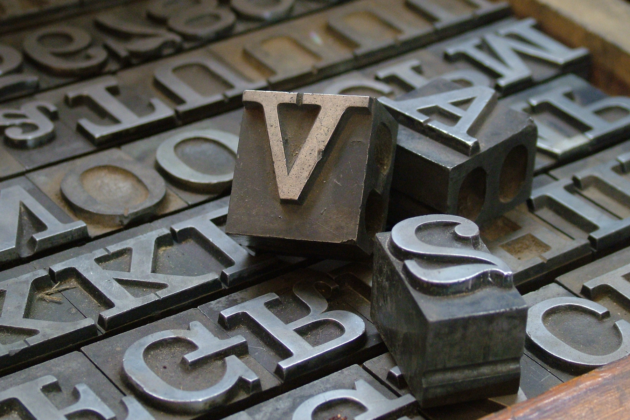
\includegraphics[width = 80mm]{fig/tipog}}
	{fonte}
	{label}
	{nota(s)}
	{legenda(s)}
\end{lstlisting}


\imagem{Titulo}{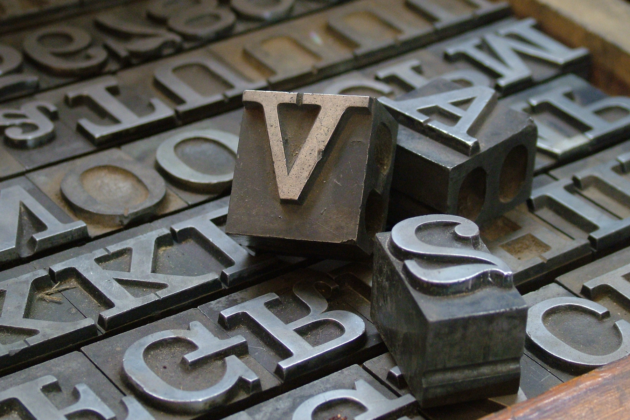
\includegraphics[width = 80mm]{fig/tipog}}{fonte}{label}{nota(s)}{legenda(s)}

Para fazer referência a esta figura é da mesma forma,\verb+\autoref{fig:label}+, \autoref{fig:label}

\subsection[Quadros e tabelas]{Quadros e tabelas}

Lembrando que quadros tem informações e são fechados lateralmente e verticalmente, tem a posição do título, fonte, nota e legenda diferentes da tabela.
\subsection[Quadros]{Inserir quadros}\label{ssec:quadros}

Para inserir um quadro são necessários 6 parâmetros:

\begin{lstlisting}
% ----------------------------------------------------------
%   Parametros
%    1 caption
%    2 elementos tabulados
%    3 fonte
%    4 qua:label
%    5 nota
%    6 legenda
\end{lstlisting}

Os elemento tabulados foram inseridos no ambiente tabular, com as laterais e parte superior e inferior fechados.

Este ambiente não quebra sua estrutura em páginas.

\begin{lstlisting}
\qquadro{Prefixos convencionados para referencias}
{\footnotesize
 \begin{tabular}{|l*{6}{|c}|}\hline
  \textbf{Elementos}:& 
       capitulos & secoes & 
       subsecoes & subsubsecoes &
       figuras   & imagens \\\hline
  \textbf{prefixos}:&
     cap &sec &
     ssec &sssec &
     fig & img\\\hline\hline
  \textbf{Elementos}:& tabelas &
     quadros & equacoes & exemplos &
     exercicios & questoes\\\hline	
  \textbf{prefixos}:&
     tab &    qua & 
     eq  &    exm & 
     exc &     que\\\hline\hline
  \textbf{Elementos}:& itens enumerados &
                       alineas&teoremas &
                       axiomas          & 
                       listagem         &\\\hline
  \textbf{prefixos}:&  inum & ali & teo & axi & lst &\\\hline
\end{tabular}}
{O autor(2021)}{quadrinho}{}{}
\end{lstlisting}

\qquadro{Prefixos convencionados para referencias}
{\footnotesize
 \begin{tabular}{|l*{6}{|c}|}\hline
  \textbf{Elementos}:& capítulos& 	seções&	subseções&	subsubseções&	
  figuras&	imagens \\\hline
  \textbf{prefixos}:&cap&sec&ssec&sssec&fig & img\\\hline\hline
  \textbf{Elementos}:&tabelas&	quadros&	
  equações& exemplos& exercícios & questões\\\hline	
  \textbf{prefixos}:&tab&qua&eq& exm & exc&que\\\hline\hline
  \textbf{Elementos}:&itens enumerados& alíneas&teoremas&	axiomas & listagem &\\\hline
  \textbf{prefixos}:&inum &ali&teo& axi &lst&\\\hline
\end{tabular}}
{O autor(2021)}{quadrinho}{}{}


A citação da fonte é feita por \verb+\citefig{bibkey}+.

Para fazer referência a este quadro, o comando \verb+\autoref{qua:quadrinho}+,\autoref{qua:quadrinho}


\subsection[Tabelas]{Inserir tabelas}

Para inserir uma tabela o comando é muito parecido, mas a normalização utilizada é o do IBGE na ABNT-UFPR.

\begin{lstlisting}
% simplificacao para colocar tabelas
% ----------------------------------------------------------
%   Parametros
%    1 caption
%    2 tabela
%    3 fonte
%    4 tab:label
%    5 nota
%    6 legenda


\tabela{T\'itulo do tabela}
{\begin{tabular}{r|c|c|c}\hline
		consumo & m\'edia & 
		m\'aximo & m\'inimo\\\hline
		& km/l& km/l& km/l\\\hline
		cidade & 11.5 & 14.8& 9.3 \\\hline
		estrada& 16.2 & 20.7& 13.4 \\\hline
\end{tabular}}
{\textcite{0230}}{exemplo}{Uma nota}{Uma legenda}
\end{lstlisting}


\tabela{T\'itulo do tabela}
{\begin{tabular}{r|c|c|c}\hline
		consumo & m\'edia & 
		m\'aximo & m\'inimo\\\hline
		& km/l& km/l& km/l\\\hline
		cidade & 11.5 & 14.8& 9.3 \\\hline
		estrada& 16.2 & 20.7& 13.4 \\\hline
\end{tabular}}
{\textcite{0230}}{exemplo}{Uma nota}{Uma legenda}


A citação da fonte é feita por \verb+\citefig{bibkey}+.

Para fazer referência a este quadro, o comando \verb+\autoref{tab:exemplo}+, \autoref{tab:exemplo}
\subsection[Equações]{Expressões matemáticas}

De preferencia ao uso do ambiente align:

\begin{lstlisting}
\begin{align}
 x + y &= 0\\
 x - y &= 2 \label{eq:2}
\end{align}
\end{lstlisting}


\begin{align}
x + y &= 0\\
x - y &= 2 \label{eq:2}
\end{align}

\subsection[Acronimos]{Siglas e símbolos}


\verb+\criarsimbolo{$\alpha$}{coeficiente de dilatação térmica}+ 

\criarsimbolo{$\alpha$}{coeficiente de dilatação térmica}, cria o símbolo e deixa anotado no texto;

\verb+\criarsigla{UFPR}{Universidade Federal do Paraná}+ 

\criarsigla{UFPR}{Universidade Federal do Paraná}\label{item:UFPR} apenas cria a sigla, sem deixar nada anotado no texto;

\verb+\criarsigla*{ABNT}{Associação Brasileira de Normas Técnicas}+ 

\criarsigla*{ABNT}{Associação Brasileira de Normas Técnicas} cria a sigla e deixa anotado no texto.

\subsection[Citações]{Citações e referências}

Para criar citações indiretas: Segundo \verb+\textcite{abntex2cite}+, \textcite{abntex2cite}.
Para criar citações indiretas: Segundo \verb+\textcite{Khaleel2018}+, \textcite{Khaleel2018}.


Para citações diretas: "[...] tudo bem quando acaba bem."\cite{abntex2cite}. \verb+\cite{abntex2cite}+


\subsubsection{Criação de referencias citadas}

Para as citações feitas para serem empregadas no texto eu customizei a separação das referências bibliográficas através de \textit{keys}.


\subsubsection{Criação de referencias consultadas}

A criação de uma bibliografia consultada após o capítulo de referências do trabalho é feita para as referências que foram utilizadas com o \textit{key}= {consulta}:

\begin{lstlisting}
....
key={consultada},
....
\end{lstlisting}  


\subsubsection{Criação de referencias de documentos não publicados ou informais}

A criação de uma bibliografia consultada após o capítulo de referências do trabalho é feita para as referências que foram utilizadas com o \textit{key}= {npub-informal}:

\begin{lstlisting}
....
key={npub-informal},
....
\end{lstlisting}  

%%%%%%%%%%%%%%%%%%%%%%%%%%%%%%%%%%%%%%%%%%%%%%%%%%%%%%%%%%%%%%%%%

no arquivo referencias.bib, no manual ABNTeX2Modelo-glossario foi adicionado a key de consulta.

\begin{lstlisting}
@Manual{abntex2modelo-glossario,
	Title = {Exemplo de uso de gloss{\'a}rio com abnTeX2},
	Author      = {abnTeX2},
	Organization= {Equipe abnteX2},
	Year        = {2013},
	Bdsk-url-1  = {http://abntex2.googlecode.com/},
	Date-added  = {2013-03-11 13:38:46 +0000},
	Date-modified={2013-04-05 11:03:36 +0000},
	Url         = {http://abntex2.googlecode.com/},
	key         = {consulta},
}
\end{lstlisting}

adicionada a chave \textit{key}={consulta} para que ele seja mencionado na lista de obras consultadas.


\subsubsection{Para fazer referência às seções ou elementos enumerados}

\begin{lstlisting}
1. Capitulos: \verb+\autoref{cha:introd}+ 

2. Secoes: \verb+\autoref{sec:util}+ 

3. Subsecoes: \verb+\autoref{ssec:imafig}+

4. Imagens: \verb+\autoref{sssec:imagem}+ 

5. Apendices: \verb+\autoref{ap:primeiroAp}+ 
          
6. Anexos: \verb+\autoref{ax:primeiroAx}+ 
          
7. Equacoes: \verb+\autoref{eq:2}+

8. Itens enumerados \verb+\autoref{item:UFPR}+ 
	
\end{lstlisting}


% PARTE DA PREPARAÇÃO DA PESQUISA
% ----------------------------------------------------------
%\part{Preparação da pesquisa}
%\input{cap02}
%

% PARTE DOS REFERENCIAIS TEÓRICOS
% ----------------------------------------------------------
%\part{Referenciais teóricos}
%\input{cap03}

% PARTE DOS RESULTADOS
% ----------------------------------------------------------
%\part{Resultados}
%\input{cap05}

% Finaliza a parte no bookmark do PDF
% para que se inicie o bookmark na raiz
% e adiciona espaço de parte no Sumário
% ----------------------------------------------------------
%\phantompart

% ---
% Conclusão (outro exemplo de capítulo sem numeração e presente no sumário)
% ---
%\chapter*[Conclusão]{Conclusão}
%\addcontentsline{toc}{chapter}{Conclusão}
% ---
%\input{cap06}

% ELEMENTOS PÓS-TEXTUAIS
% ----------------------------------------------------------
\postextual

% Ajuste vertical do titulo de referencias no sumário
% ----------------------------------------------------------
\addtocontents{toc}{\vspace{-24pt}}

% Referências bibliográficas
% ----------------------------------------------------------
%\bibliography{referencias}

\begingroup

\printbibliography[heading=bay, notkeyword= {consulta}, notkeyword={npub-informal}]
  
\endgroup

% ----------------------------------------------------------

% Ajuste vertical dos titulos dos capitulos postextuais
% ----------------------------------------------------------
\addtocontents{toc}{\vspace{-12pt}}

% Glossário
% ----------------------------------------------------------
% Consulte o manual da classe abntex2 para orientações sobre o glossário.
%
%\glossary

% Apêndices
% ----------------------------------------------------------
\ifthenelse{\equal{\terApendice}{Sim}}
{\begin{apendicesenv}

        % Numeração arábica para os apêndices
        % --------------------------------------------------
        \renewcommand{\thechapter}{\arabic{chapter}}
        % Imprime uma página indicando o início dos apêndices
        % \partapendices

        % Existem várias formas de se colocar anexos.
        % O exemplo abaixo coloca 2 apêndices denominados de 
        % DESENVOLVIMENTO DETALHADO DA PINTURA e 
        % ESCOLHA DO MATERIAL DE IMPRESSÃO:
        % ---
        % --- insere um capítulo que é tratado como um apêndice
        %\chapter{DESENVOLVIMENTO DETALHADO DA PINTURA}
        % 
        %\lipsum[29] % gera um parágrafo
        %
        % --- insere um capítulo que é tratado como um apêndice
        %\chapter{ESCOLHA DO MATERIAL DE IMPRESSÃO}
        % 
        %\lipsum[30] % gera um parágrafo

        % --- Insere o texto do arquivo ap01.tex
        % 
        % --- O conteúdo do arquivo pode ser vários anexos ou um único apêndices.
        %     A vantagem de se utilizar este procedimento é de suprimi-lo
        %     das compilações enquanto se processa o resto do documento.

        % --- insere um capítulo que é tratado como um apêndice
\label{ap:ap01}
\poschap{ESCOLHA DO MATERIAL}

\lipsum[30] % gera um parágrafo
\section*{Testes se\c{C}\~aO}

\lipsum[22] % gera um parágrafo

\end{apendicesenv}
}{}


% Anexos
% ----------------------------------------------------------
\ifthenelse{\equal{\terAnexo}{Sim}}{
\begin{anexosenv}

        % Numeração arábica para os apêndices
        % --------------------------------------------------
        \renewcommand{\thechapter}{\arabic{chapter}}
        % --- Imprime uma página indicando o início dos anexos
        % \partanexos

        % Existem várias formas de se colocar anexos.
        % O exemplo abaixo coloca 2 anexos denominados de 
        % TABELA DE VALORES e GRÁFICOS DE BALANCEMANTO:
        % ---
        % --- insere um capítulo que é tratado como um anexo
        %\chapter{TABELAS DE VALORES}
        % 
        %\lipsum[31] % gera um parágrafo
        %
        % --- insere um capítulo que é tratado como um anexo
        %\chapter{GRÁFICOS DE BALANCEAMENTO}
        % 
        %\lipsum[32] % gera um parágrafo

        % --- Insere o texto do arquivo ax01.tex
        % 
        % --- O conteúdo do arquivo pode ser vários anexos ou um único anexo.
        %     A vantagem de se utilizar este procedimento é de suprimi-lo
        %     das compilações enquanto se processa o resto do documento.

         % --- insere um capítulo que é tratado como um apêndice
\poschap{anexando ESCOLHA DO MATERIAL}
   
\lipsum[30] % gera um parágrafo
   \section*{anexando testes secao} 
\end{anexosenv}
}{}

% INDICE REMISSIVO
%---------------------------------------------------------------------
\ifthenelse{\equal{\terIndiceR}{Sim}}{
\phantompart
\printindex
}{}

\end{document}
